\section{Chapter 2: Learning a Neural Field of Text Representations using Satellite Images}
\label{sec:sat2cap}
Dhakal, Aayush, et al. ``Sat2cap: Mapping fine-grained textual descriptions from satellite images." \textit{IEEE/ISPRS Workshop: Large Scale Computer Vision for Remote Sensing (Best Paper EARTHVISION) 2024.}
\subsection{Overview}
In the previous chapter, we proposed a framework to learn a general-purpose neural field over the earth. In this chapter, we will learn a specialized neural field of text-aligned representations. For any location $(lat,lon)$, we want to learn a function $R= F_\theta(lat,lon)$, where $R$ captures the fine-grained text describing the query location. Instead of directly using the geolocation coordinates as input to the neural field, we use a satellite image as a proxy for the location, i.e., $ R = F_\theta(Img(lat, lon))$.

Modeling the relationship between text and images is a well-studied problem in deep learning. Models such as CLIP~\cite{radford2021learning} and ALBEF~\cite{li2021align} are trained on a large database of captioned images to learn a multimodal embedding space that unifies vision and text. However, we observe that directly using these models on satellite imagery leads to the collapse of representations into a few coarse textual concepts, such as city, beach, and island. Satellite images capture a broad perspective of a geolocation but offer limited insight
into the intricate concepts and dynamics within the location. Hence, directly using overhead images with such models would only allow us to learn coarse-level textual concepts.

One solution is to train a model using satellite images and fine-grained captions of those locations. However, such datasets do not exist in large-scale. To address this issues, we exploit the cross-view relation of satellite images with corresponding ground-level images. Specifically, we propose a weakly-supervised
cross-view approach for learning fine-grained textual concepts for geographic locations by leveraging co-located ground-level images. We create a large-scale dataset with paired overhead and ground-level images. We then train a model that aligns overhead images with ground-level images in the CLIP space. Our training leverages an emergent behaviour, where aligning the overhead images with ground-level images, as a by-product, aligns them with the corresponding text descriptions of the ground-level images. This allows us to learn a fine-grained vision-language representation space for satellite images in the absence of text data.  

\begin{equation}
    G_i = f_\theta{(g_i)}
\end{equation}
\begin{equation}
    O_i = g_\theta{(o_i)}
\end{equation}    

To align the overhead image embeddings with the ground-level CLIP embeddings, we contrastively train our model using the InfoNCE~\cite{oord2018representation} loss as follows:
%
\begin{equation}
    L = \frac{1}{k}\sum_{i=0}^{k} -\log\frac{exp(O_i \cdot G_i / \tau)}{\sum_{j=0}^{k} exp(O_i \cdot G_j / \tau) }
\end{equation}

\begin{figure*}[!t]
\begin{center}
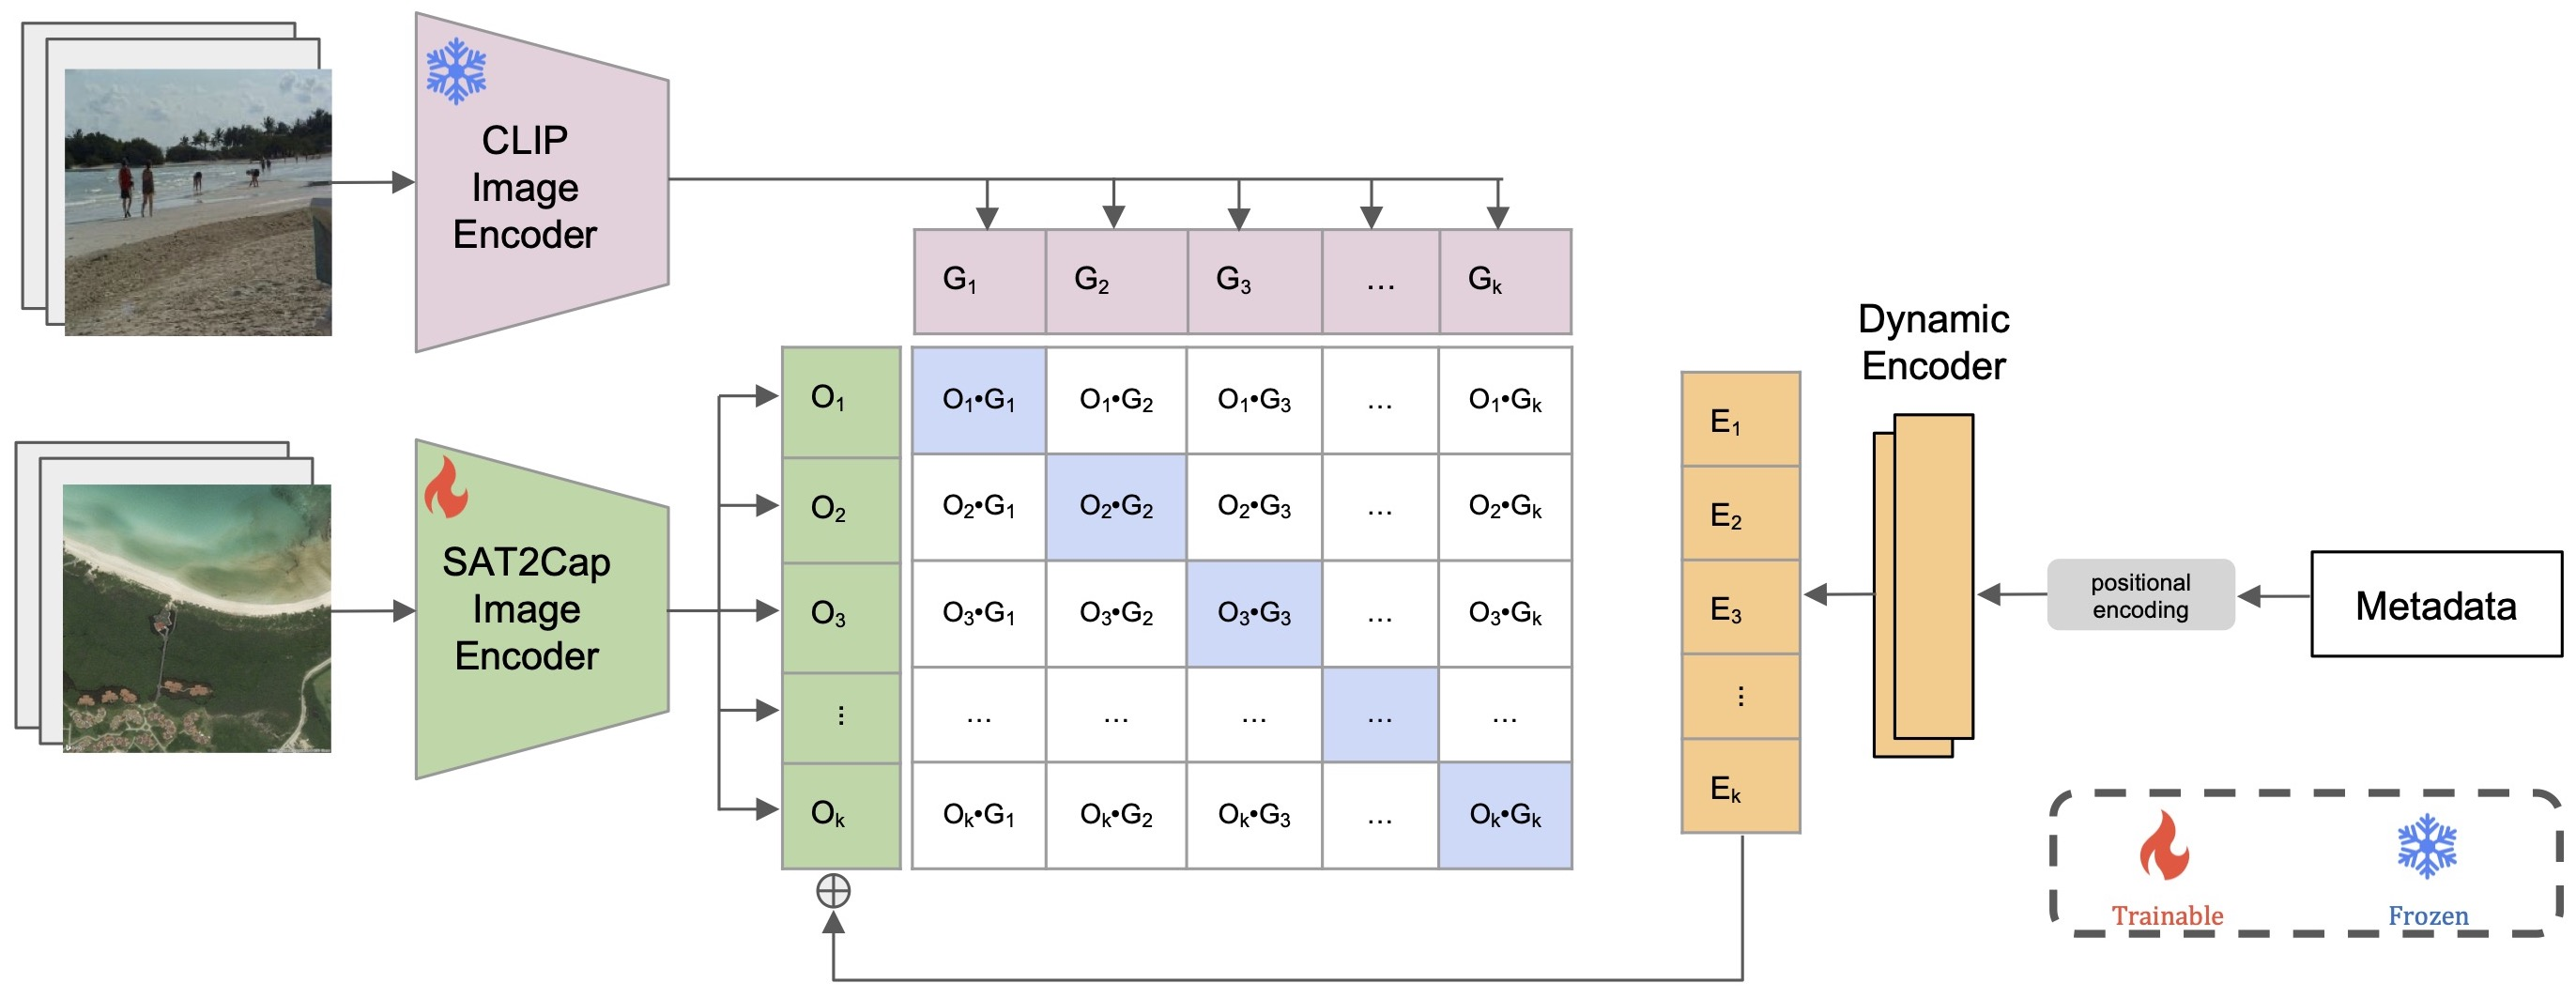
\includegraphics[width=\linewidth, scale=0.3]{proposal/images/framework.jpg}
\end{center}
   \caption{\textbf{Sat2Cap Framework:} The frozen CLIP Image Encoder takes as input the ground-level images and generates their CLIP embeddings. The trainable Sat2Cap Image Encoder takes as input the overhead images, and the Dynamic Encoder takes as input the date, time, and location information. The respective overhead image embeddings and meta-information embeddings are added element-wise, and the resulting embeddings are contrastively trained with the CLIP embeddings of the ground-level images.}  
\label{fig:Sat2Cap}
\end{figure*}
\subsection{Method}
\label{sec:method}
Our objective is to learn an embedding space that describes the expected ground-level scene given a geographic location and an overhead image. We have ground-level images $\{g_1, g_2, ...g_n\}$, corresponding overhead images $\{o_1, o_2, ...o_n\}$, and respective metadata for the ground-level images $\{e_1, e_2, ...e_n\}$. Each $e_i$ contains the latitude and longitude information of the sample, as well as the date and time for when the ground-level image was captured. We also have a CLIP image encoder $f_{\theta}$ that generates CLIP embeddings for a given ground-level image.

\subsubsection{Dataset}
\label{dataset}
We created a large-scale cross-view dataset to train our model. The ground-level images in the dataset are taken from the YFCC100M~\cite{thomee2016yfcc100m} dataset. The YFCC100M dataset contains 99.3 million images, which are collected from Flickr. Our cross-view dataset uses a smaller sample from this collection which excludes all US imagery. We filter out all images that are not geotagged. The resulting dataset contains 6.1M images. Each of these images has a geolocation, timestamp, and other meta-information. For each image, we download an overhead image centered at its location. Specifically, we use the Bing Maps API to download $800$x$800$ patch satellite images at $0.6m/px$ resolution. We randomly sampled 100k images to be used for testing.

\newcommand{\cmark}{\ding{51}}%
\newcommand{\xmark}{\ding{55}}%

\begin{table}
 \begin{center}
 \small
 \resizebox{\linewidth}{!}{
    \begin{tabular}{c c c c |c c c|c c c}
 \hline
 \multicolumn{4}{c|}{Method} &
 \multicolumn{3}{c|}{Overhead2Ground (10K)} &
 \multicolumn{3}{c}{Ground2Overhead (10K)} \\
 
 \hline
 Model &Meta/Training &Dropout & Meta/Inference & R@5$\uparrow$ & R@10$\uparrow$ & Median-R$\downarrow$ & R@5$\uparrow$ & R@10$\uparrow$ & Median-R$\downarrow$\\
 \hline
 CLIP & - &- & - & 0.007 & 0.013 & 1700 & 0.108 & 0.019 & 2857 \\
 \hline
 \multirow{4}{2em}{ours} & \xmark & \xmark & \xmark & 0.398 & 0.493 & 15 & 0.356 & 0.450 & 11\\
 & \cmark & \xmark & \xmark & 0.322 & 0.413 & 34 & 0.254 & 0.343 & 20\\
 & \cmark& \xmark & \cmark & 0.368 & 0.467 & 23 & 0.298 & 0.398 & 13\\
 & \cmark& \cmark & \xmark & 0.467 & 0.564 & 13.5 & 0.366 & 0.462 & 7\\
 & \cmark& \cmark & \cmark & \textbf{0.493} & \textbf{0.591} & \textbf{12} & \textbf{0.390} & \textbf{0.482} & \textbf{6}\\


\end{tabular}
}
\end{center}
  \caption{\textbf{Cross-view retrieval performance of Sat2Cap model:} The table shows that CLIP performs poorly for the task of cross-view retrieval. Moreover, we study the performance of our model under various settings. The \textbf{Meta/Training} column ablates the impact of adding meta-information in training. The \textbf{Dropout} column ablates the impact of randomly dropping out the Dynamic Encoder in training. The \textbf{Meta/Inference} column ablates the impact of adding meta-information in inference. Our experiments show that using all three achieves the best performance.}
\label{table:retrieval}
\end{table}

\subsubsection{Approach}
We initialize our Sat2Cap image encoder $g_\theta$ with the weights of $f_\theta$. A batch of ground-level images $\{g_1, g_2, ..., g_k\}$ is passed through the CLIP encoder to get the ground-level CLIP embeddings. These embeddings serve as the target for alignment. A batch of corresponding overhead images $\{o_1, o_2, ..., o_k\}$ is passed through the Sat2Cap image encoder to obtain the respective embeddings:  
%
We also keep a queue $Q$ and fill it with CLIP embeddings of ground images. Here, $|Q|>>k$ and the embeddings from the queue are used as additional negative samples for our contrastive objective. As in MoCo~\cite{he2020momentum}, the queue is continuously updated during the training with the most recent batch. Minimizing this objective minimizes the distance between co-located overhead and ground-level images in the CLIP space. It is worth noting that throughout the training process, the CLIP image encoder is frozen. Hence, with our training procedure, we allow the overhead images to move close to images from their respective ground-level scene in the CLIP space. As a byproduct, the overhead images also move closer to the textual descriptions of ground-level images, which we are ultimately interested in mapping.

\begin{figure*}[!t]
\begin{center}
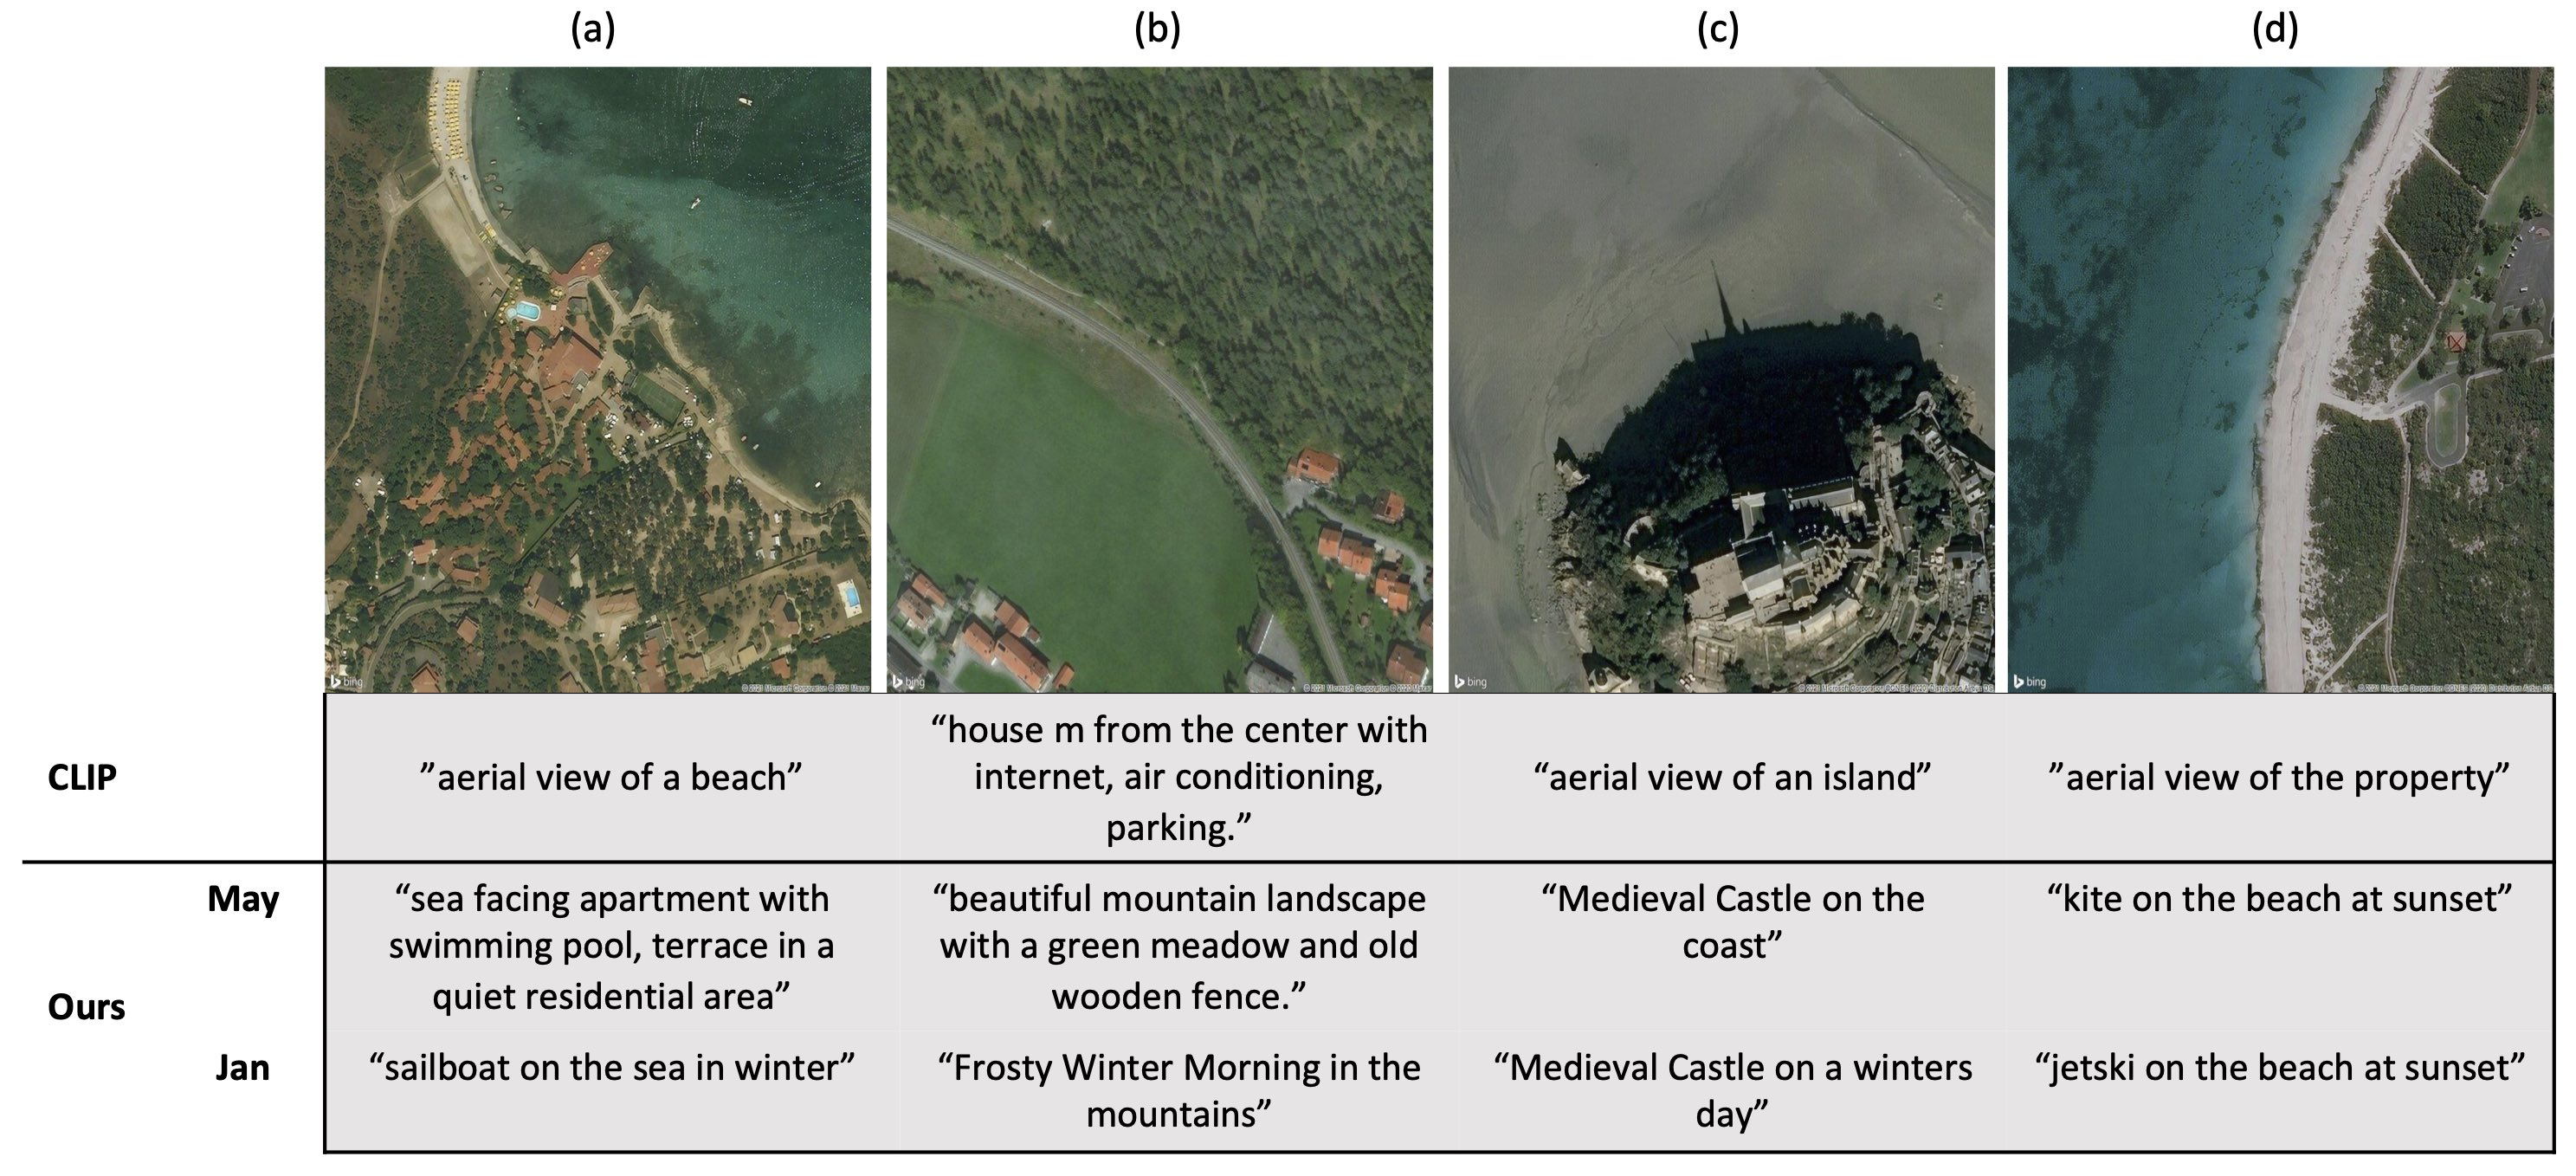
\includegraphics[width=0.95\linewidth]{proposal/images/caption_gen_2.jpg}
\end{center}
   \caption{Captions generated by the CLIPCAP model \cite{mokady2021clipcap} using CLIP embeddings vs.\ Dynamic Sat2Cap embeddings. (Row-1) shows the results from CLIP embeddings, which produce many generic descriptions. (Row-2 and 3) show the results from our Sat2Cap embeddings for the month of May and January, respectively. The captions generated using Sat2Cap embeddings are more fine-grained and dynamic. While (d) does not add any winter properties for the January query, this behavior is expected as the image is over Australia, where January falls in the middle of summer.}    
\label{fig:img1}
\end{figure*}

\begin{figure*}[!t]
    \centering
    % First subfigure
    \begin{subfigure}{}
        \centering
        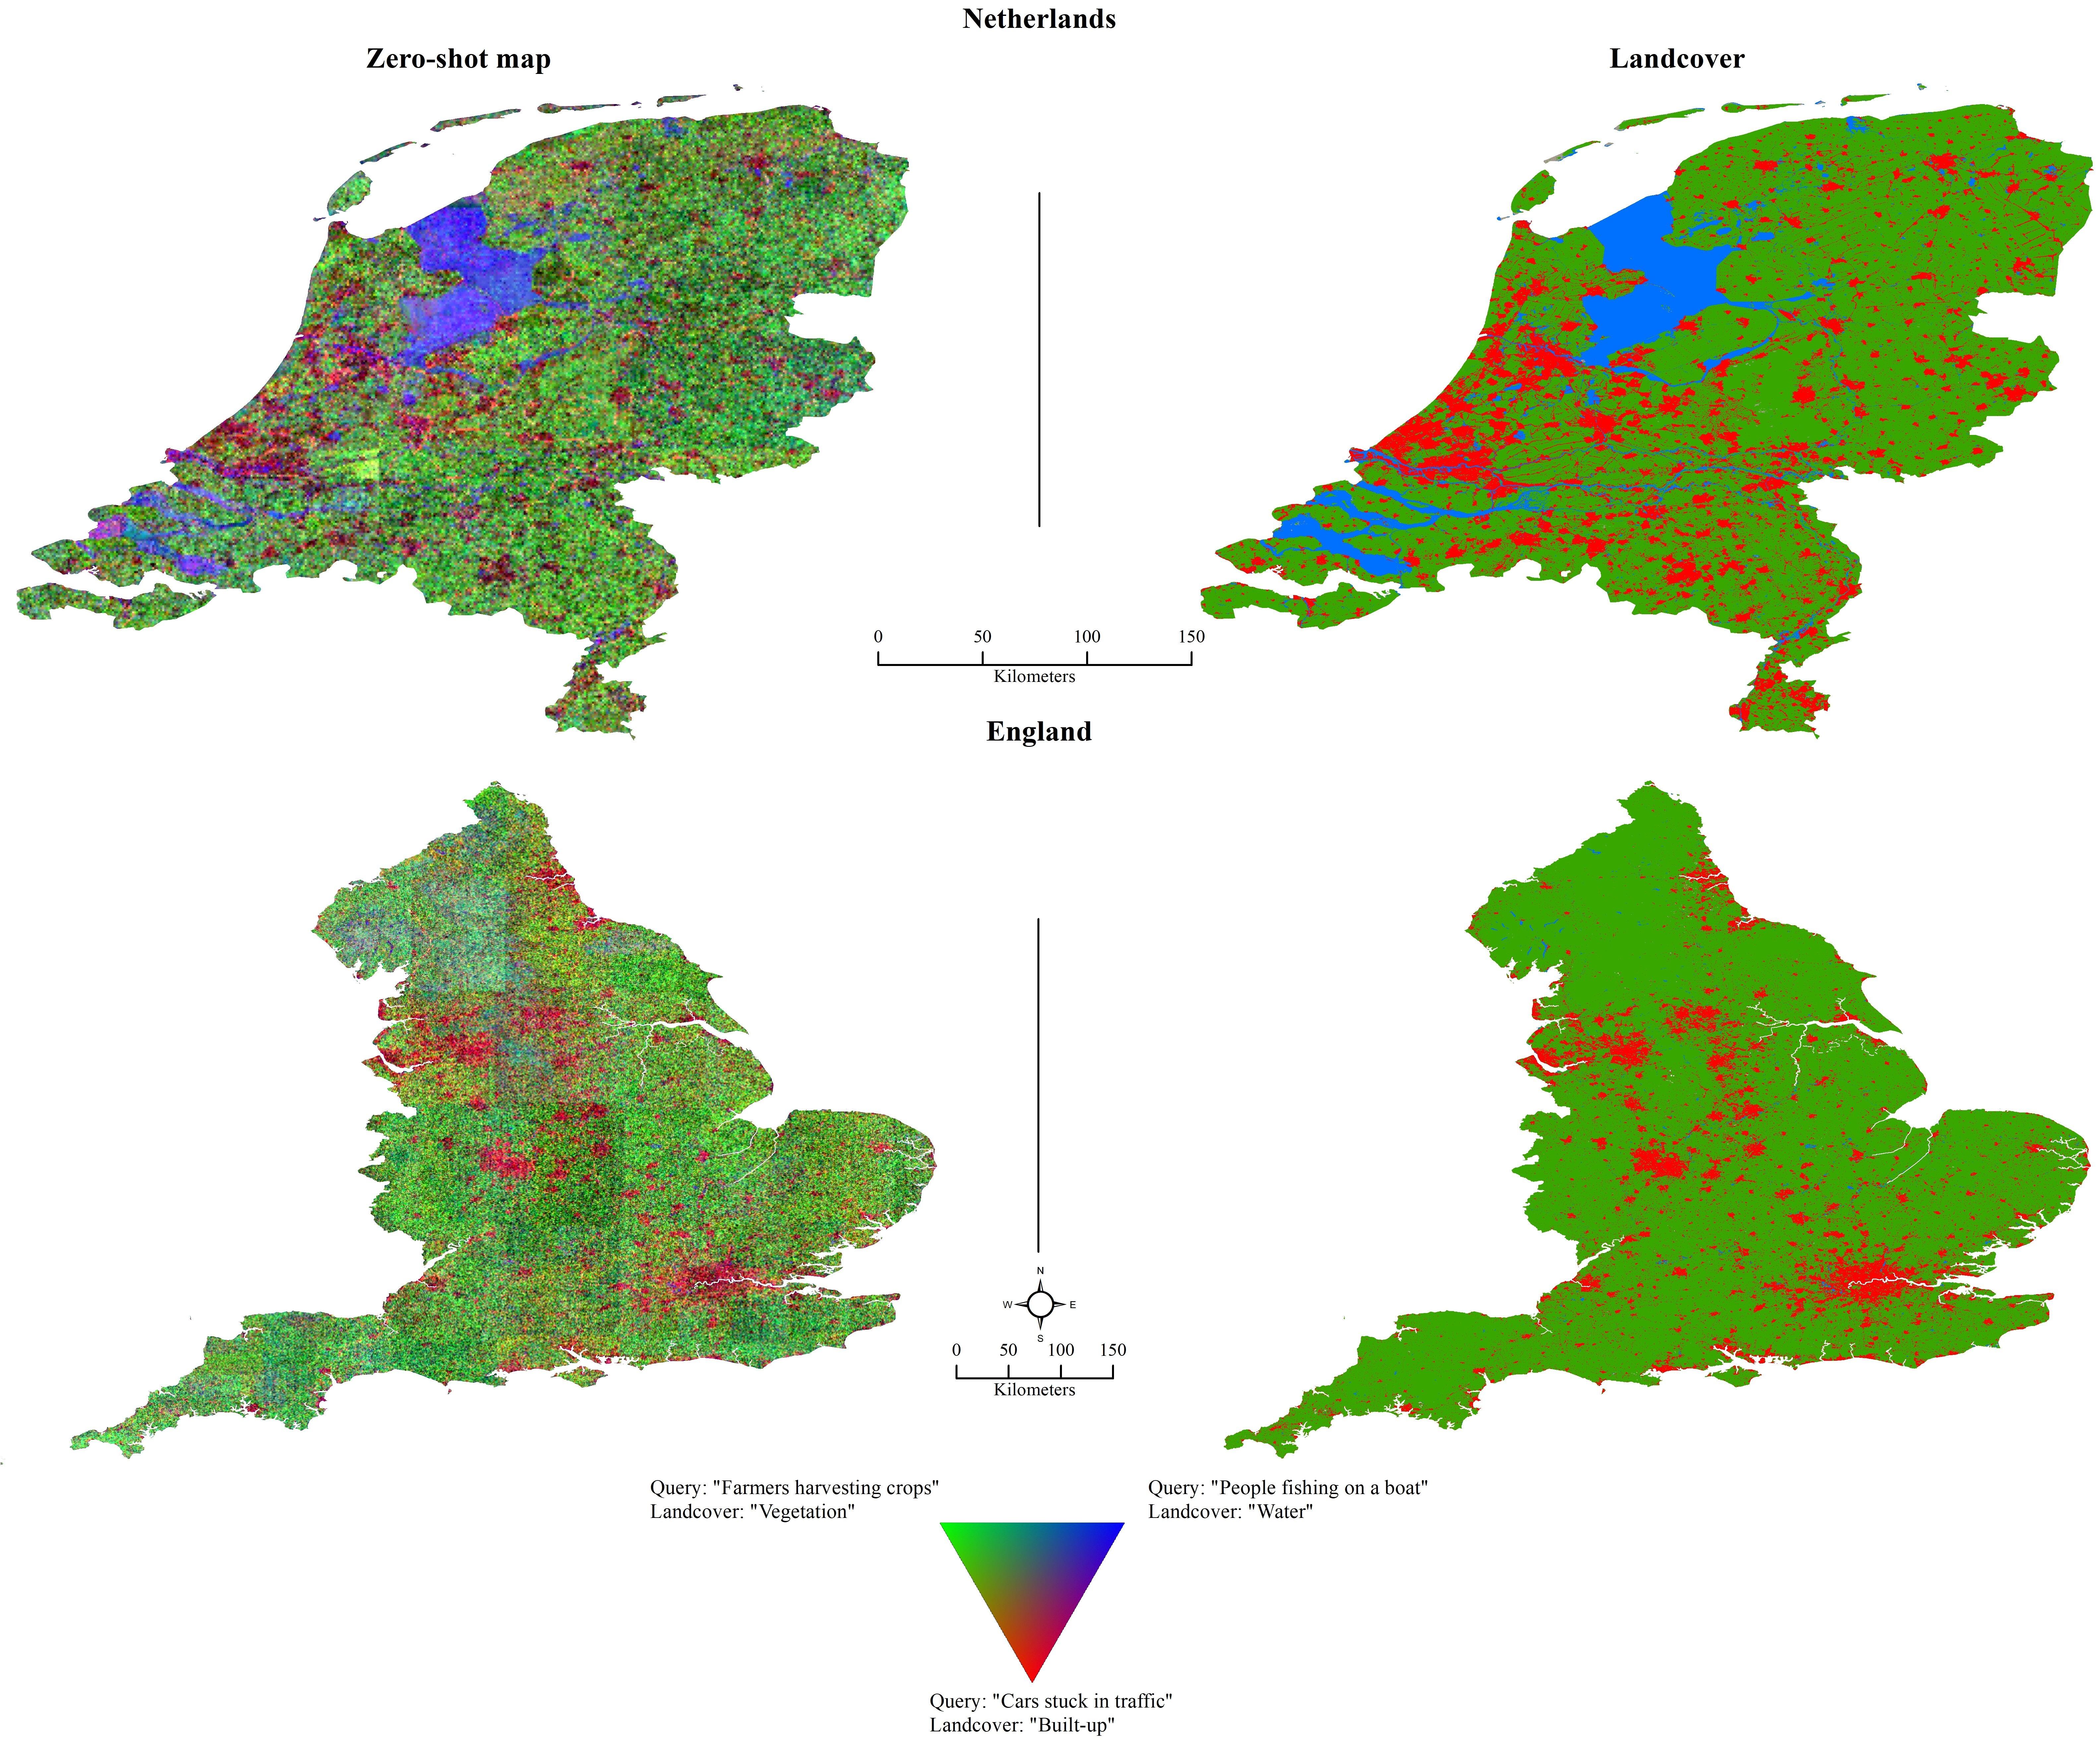
\includegraphics[width=\linewidth,height=0.5\textheight,keepaspectratio]{proposal/images/rgb_map.jpg}
        \caption{\textbf{Country-level maps of textual descriptions}: (Col 1-2) shows the country-level maps created using Sat2Cap for three prompts: ``Cars stuck in traffic," ``People fishing on a boat," and ``Farmers harvesting crops." We compare the predicted zero-shot maps with landcover maps of the region.}
        \label{fig:generic_maps}
    \end{subfigure}
    \vskip 0.5em
    % Second subfigure
    \begin{subfigure}{}
        \centering
        \includegraphics[width=\linewidth,height=0.4\textheight,keepaspectratio]{proposal/images/ams_road.jpg}
        \caption{\textbf{Fine-grained maps CLIP vs Sat2Cap:} We create zero-shot maps on a city level using CLIP and Sat2Cap for two prompts: ``Heavy trucks transporting goods" and ``People waking in the streets of downtown." Compared to CLIP, Sat2Cap activations are more localized to the appropriate regions for a given prompt. Sat2Cap is better at distinguishing between fine-grained concepts like \textbf{highway} and \textbf{downtown street}.}
        \label{fig:fg_maps}
    \end{subfigure}
    \label{fig:maps_combined}
\end{figure*}
\subsubsection{Learning Dynamic Concepts of Places}

Many ground-level concepts are temporally dependent. Concepts like ``crowded street", or ``snowy place" can dramatically vary based on the exact time we query about them. To model such dynamic concepts, we condition Sat2Cap on the timestamps of the ground-level images.

For each sample, we extract the year, month, day, and hour in which the ground image was taken. We also add the geolocation information to provide a stronger signal to the model. We encode this meta-information using sin-cos encoding and pass it through a shallow, fully connected network, which we call the Dynamic Encoder $(h_\theta)$. The output from $h_\theta$ is added element-wise to the output from the Sat2Cap encoder before computing the objective.

\begin{equation}
    S_i = O_i + E_i
\end{equation}
where $O_i$ is the output from the Dynamic Encoder. Now the objective function changes to:
\begin{equation}
\label{eq:finaleq}
   L_{dynamic} = \frac{1}{k}\sum_{i=0}^{k} -\log\frac{exp(S_i \cdot G_i / \tau)}{\sum_{j=0}^{k} exp(S_i \cdot G_j / \tau) } 
\end{equation}
where $S_i$ is the sum of outputs from the Image Encoder and Dynamic Encoder 

Our complete framework is shown in Figure~\ref{fig:Sat2Cap}. To prevent overfitting to the meta-information, we implement random dropout of the Dynamic Encoder during training. Our experiments from Section~\ref{sec:sat2cap_results} show that this addition significantly improves the performance of our model.

\subsection{Results}
\label{sec:sat2cap_results}
Our model learns a powerful geo-text embedding space that can be used for a variety of applications. We describe three experiments to demonstrate the efficacy of our model.
\subsubsection{Cross-View Image Retrieval}
In this experiment, we show that our model learns a strong relationship between co-located overhead images and ground images in the CLIP space. We randomly sample 10,000 image pairs from the test set for this experiment. First, we predict the Sat2Cap embeddings for all overhead images and the corresponding CLIP embeddings for all the ground-level images in the test set. We then compute top-k (or R@k) and median rank metrics between the Sat2Cap overhead embeddings and the CLIP ground embeddings. The top-k metric measures how often the ground truth falls within the top-k closest images for a given query image. Table~\ref{table:retrieval} shows the cross-view retrieval results.

Our results highlight that CLIP space, in itself, is remarkably poor at learning the relationship between a location and the corresponding ground-level scene. The low cross-view retrieval scores imply that we cannot accurately reason about ground-level scene using the CLIP embeddings of co-located overhead images. On the other hand,  the high cross-view retrieval scores of Sat2Cap suggest that the Sat2Cap embedding of a location approximates the CLIP embeddings of the images at the ground-level. This ultimately results in an emergent alignment between location and textual descriptions of the ground level.
\subsubsection{Fine-grained and Dynamic Caption Generation}
To generate captions from our embeddings, we use the CLIPCap~\cite{mokady2021clipcap} model. CLIPCap allows us to generate captions by learning a mapping from the CLIP space to the text space. Figure~\ref{fig:img1} shows qualitative examples of captions generated by passing CLIP embedings vs Sat2Cap embeddings as input for a given overhead image. We observe that when using CLIP embeddings of the overhead images as input, the captions generated by CLIPCap mostly describe generic concepts of a location like a beach, island, property, etc. In contrast, our Sat2Cap embeddings produce more fine-grained and aesthetically pleasing captions. Furthermore, we use the dynamic encoder to generate captions in two different months, for the same location.

\subsubsection{Zero-Shot Map of Fine-grained Concepts}
We use Sat2Cap embeddings to create zero-shot maps using fine-grained prompts. To do this, we choose a region and download high-resolution satellite images $(0.6m/px)$ over the region. We precompute the Sat2Cap embeddings for all the images. At inference time, for a given text query, we predict the CLIP embedding and compute its similarity with the overhead image embeddings. The process of computing the similarities only takes about 4 seconds. Figure~\ref{fig:generic_maps} and Figure~\ref{fig:fg_maps} show zero-shot maps at country-scale and city-scale data.

\subsection{Proposed Direction}
We are also working on follow-up of Sat2Cap. Sat2Cap leveraged pre-trained vision-language models to learn the correspondence between satellite images and ground-level image descriptions. One key limitation of this approach is that it learns a single ground-level concept/embedding/descriptor for a given satellite image, resulting in coarse-grained information. We are currently working on Sat360, a framework that learns the correspondence between satellite image and ground-level image descriptions conditioned on a viewing direction. More specifically, Sat360 allows learning fine-grained text for specific regions within a satellite image, which was not possible using Sat2Cap. Our key insight is that explicitly aligning viewing orientation by pairing directional crops from street view panoramas with their corresponding masked regions in overhead imagery, achieves pixel-level correspondence without manual annotations. By leveraging the joint vision-language space, Sat360 enables zero-shot tasks such as fine-grained cross-view retrieval, orientation estimation, and open-vocabulary aerial segmentation. We are currently working on Sat360 and plan to submit a paper on November. 

\subsection{Chapter Conclusion}
In this chapter, we proposed a specialized neural field of textual representations. We presented a weakly supervised framework for learning a semantically rich embedding space between geolocation and fine-grained text. For this task, we leveraged the unique property of satellite images i.e. relation of satellite images with corresponding ground-level images. By leveraging this property, we were able to learn a foundational vision-language model without using any text. We demonstrated that our framework can efficiently generate high-quality zero-shot maps from fine-grained text prompts. Thus, we demonstrated that it is possible to develop efficient learning algorithms, by understanding the unique properties of the input modality and incorporating those insights into our models. 


